\documentclass[12pt, a4paper]{article}

% Paquetes necesarios
\usepackage[utf8]{inputenc}
\usepackage[spanish]{babel}
\usepackage{graphicx}
\usepackage{geometry}
\usepackage{float}
\usepackage{booktabs} % Para tablas más profesionales
\usepackage{hyperref}

% Configuración de márgenes
\geometry{top=2.5cm, bottom=2.5cm, left=3cm, right=3cm}

% Título y autor
% Título y autor modificados
\title{
    \vspace{-1.5cm} % Ajusta este valor si el encabezado sube o baja demasiado
    \begin{center}
        {\Large \textbf{UNIVERSIDAD NACIONAL MAYOR DE SAN MARCOS}}\\[0.2cm]
        {\small \textbf{(Universidad del Perú, DECANA DE AMÉRICA)}}\\[0.8cm]
        {\large \textbf{FACULTAD DE CIENCIAS MATEMÁTICAS}}\\[0.2cm]
        {\large \textbf{ESCUELA PROFESIONAL DE COMPUTACIÓN CIENTÍFICA}}\\[1cm]
        
        \begin{tabular}{@{}l@{}}
            \textbf{Asignatura:} Redes, Arquitectura y Comunicaciones \\
            \textbf{Docente:} Mg. Jaime Rubén Pariona Quispe \\
        \end{tabular}
        
        \vspace{0.8cm}
        
        \begin{tabular}{@{}l@{}}
            \textbf{Integrantes:} \\
            1. Huayta Huillcahuare, Luis Enrique \\
            2. Salvador Damián, Navarro \\
            3. Yalo Palomino, Nicanor  \\
        \end{tabular}
        
        \vspace{1.5cm}
        
        {\Large Tarea N° 3: \textbf{Diseño e Implementación de Red LAN Multinivel con Segmentación por Laboratorios}}
    \end{center}
}
\author{} % Se deja vacío porque el autor ya está incluido en el título
\date{\today}
\begin{document}

% ---------------------------------------------------------
% PÁGINA 1: Imagen a página completa
% ---------------------------------------------------------
\begin{figure}[p]
    \centering
    % Reemplaza 'topologia_packet_tracer.png' por el nombre exacto de tu primera imagen
    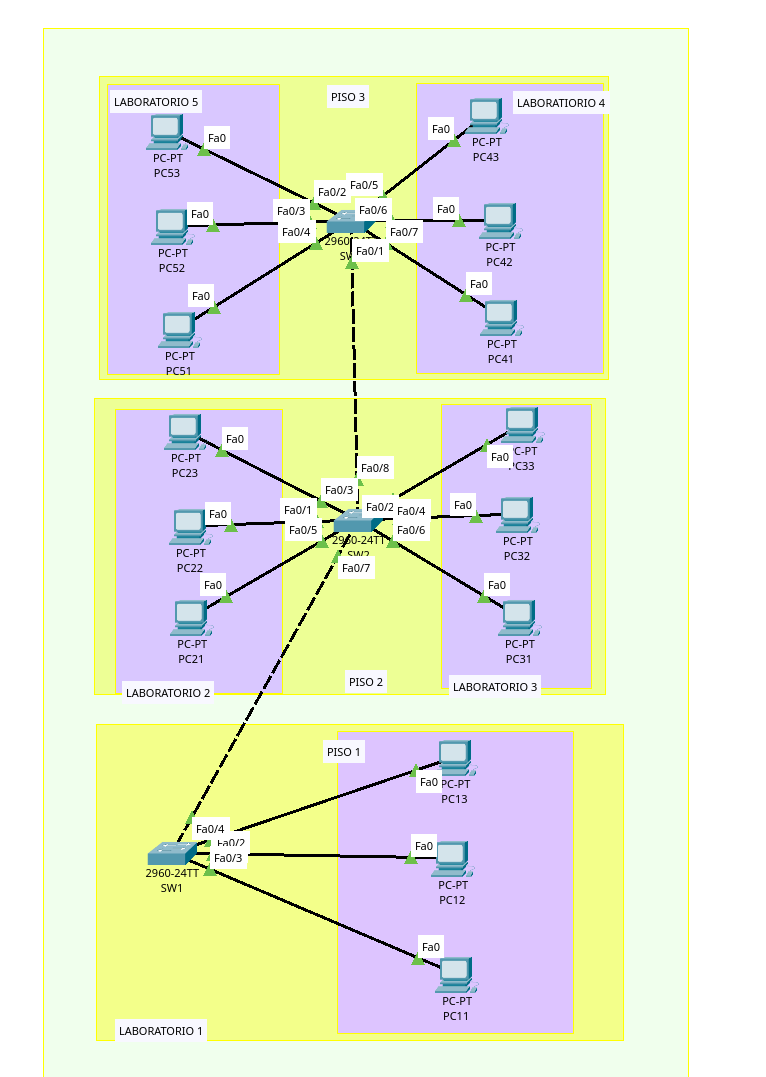
\includegraphics[width=1.15\textwidth, height=0.99\textheight, keepaspectratio]{redes_tarea3.png}
    \caption{Topología física y lógica de la red implementada en Cisco Packet Tracer.}
    \label{fig:topologia}
\end{figure}
\thispagestyle{empty} % Opcional: quita el número de página en la portada de la imagen

\newpage

% ---------------------------------------------------------
% PÁGINA 2 y 3: Contenido del Informe
% ---------------------------------------------------------
\maketitle

\section{Introducción}
El presente informe detalla el diseño, la asignación de direccionamiento lógico y la metodología de verificación de una red de área local (LAN) implementada en un edificio de tres pisos. La topología, representada en la Figura \ref{fig:topologia}, sigue un modelo jerárquico donde cada piso cuenta con un switch central (Cisco 2960-24TT) que interconecta los diferentes laboratorios de computación. Los switches de cada piso se enlazan entre sí mediante enlaces troncales para conformar una red unificada, permitiendo la comunicación entre todos los nodos finales.

\section{Diseño de Direccionamiento IP}
Con base en el esquema de red proporcionado y los requerimientos establecidos, se ha definido un direccionamiento IP bajo la red base \textbf{192.168.1.0/24}. Para garantizar la organización y facilitar la administración, se ha optado por segmentar los rangos de direcciones IP asignando un bloque específico a cada laboratorio. 

El direccionamiento se ha generado respetando los rangos indicados en el diseño, utilizando el último octeto para identificar tanto el laboratorio como el host. Se asume que la puerta de enlace (Gateway) predeterminada para todos los dispositivos es la dirección \textbf{192.168.1.1}, dejando el rango de \textbf{192.168.1.2 a 192.168.1.255} para hosts finales, de acuerdo con lo estipulado en el diseño original.

A continuación, se presenta la tabla de asignación de direcciones IP por laboratorio:

\begin{table}[H]
    \centering
    \caption{Asignación de rangos IP por Laboratorio}
    \label{tab:ips}
    \begin{tabular}{@{}llll@{}}
        \toprule
        \textbf{Piso} & \textbf{Laboratorio} & \textbf{Rango de IPs} & \textbf{Máscara de Subred} \\ \midrule
        Piso 1 & Laboratorio 1 & 192.168.1.11 - 192.168.1.19 & 255.255.255.0 \\
        Piso 2 & Laboratorio 2 & 192.168.1.21 - 192.168.1.29 & 255.255.255.0 \\
        Piso 2 & Laboratorio 3 & 192.168.1.31 - 192.168.1.39 & 255.255.255.0 \\
        Piso 3 & Laboratorio 4 & 192.168.1.41 - 192.168.1.49 & 255.255.255.0 \\
        Piso 3 & Laboratorio 5 & 192.168.1.51 - 192.168.1.59 & 255.255.255.0 \\ \bottomrule
    \end{tabular}
\end{table}

\section{Metodología de Verificación}
Para validar el correcto funcionamiento de la red y asegurar que el enrutamiento y la conectividad se establecen adecuadamente, se define un plan de pruebas de conectividad. El requisito fundamental es que \textbf{las verificaciones se realicen entre computadoras de diferentes laboratorios}, lo que garantiza que el tráfico no solo se conmuta localmente en un switch, sino que atraviesa los enlaces troncales entre pisos.

\subsection{Pruebas de Conectividad (Ping)}
Se utilizará la herramienta \texttt{ping} de ICMP para verificar la comunicación extremo a extremo. A continuación, se detallan los pasos para una prueba representativa:

\begin{enumerate}
    \item \textbf{Origen:} PC11 (Laboratorio 1, Piso 1) con IP 192.168.1.11.
    \item \textbf{Destino:} PC31 (Laboratorio 3, Piso 2) con IP 192.168.1.31.
    \item \textbf{Procedimiento:} Desde la terminal de PC11, ejecutar el comando: \texttt{ping 192.168.1.31}.
    \item \textbf{Resultado Esperado:} Se deben recibir respuestas ICMP exitosas (Reply from 192.168.1.31). Esto comprueba la comunicación a través de SW1 hacia SW2.
\end{enumerate}

\begin{figure}[H]
    \centering
    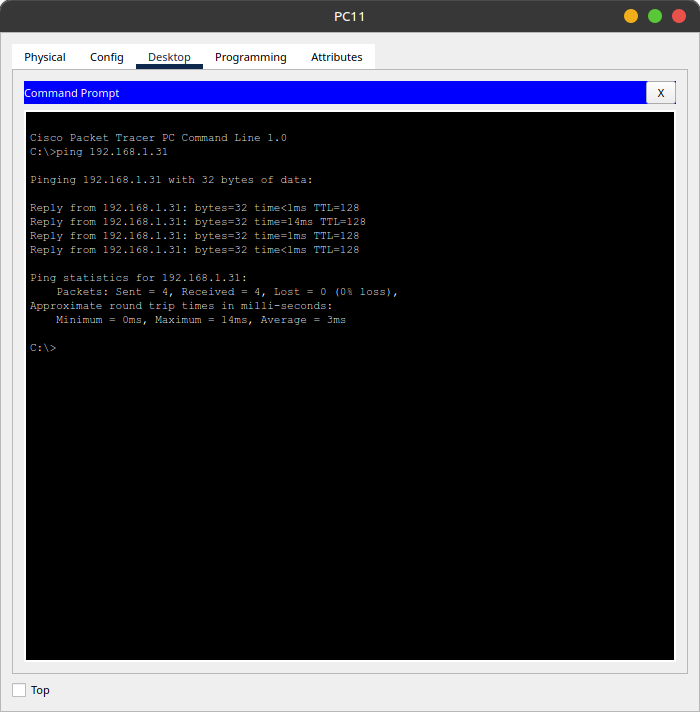
\includegraphics[width=0.8\linewidth]{ping.png}
    \caption{Prueba de conectividad exitosa (ping) desde la PC11 del Laboratorio 1 hacia la dirección 192.168.1.31 del Laboratorio 3.}
    \label{fig:placeholder}
\end{figure}
De manera análoga, se deben realizar pruebas cruzadas entre todos los laboratorios (por ejemplo, Lab 1 con Lab 4, Lab 2 con Lab 5, etc.). Si alguna prueba falla, se debe verificar la configuración de las interfaces, el estado de los enlaces troncales (up/up) y las tablas de enrutamiento o VLANs si aplican.

\section{Conclusión}
El diseño propuesto cumple con los requerimientos de segmentación lógica mediante la asignación de rangos IP específicos por laboratorio, facilitando la identificación de fallas y la aplicación de políticas de seguridad. La topología en estrella jerárquica implementada en Packet Tracer permite una escalabilidad sencilla y la verificación cruzada mediante comandos \texttt{ping} asegura la interoperabilidad de toda la infraestructura de red del edificio.

\end{document}